% Use this if you generate the presentation itself.
\documentclass[%
final,
xcolor = table,
usenames,
dvipsnames,
table,
aspectratio = 169]{beamer}

% Use this documentclass line for generating the handout
% \documentclass[%
% final,
% xcolor = table,
% usenames,
% dvipsnames,
% table,
% hadout,
% draft,
% aspectratio = 169,
% ]{beamer}

\usepackage{appendixnumberbeamer}

% minted load packages: keyval, ifthen, etoolbox, kvoptions, calc, xstring,
% fancyvrb, ifplatform, xcolor, float, pdftexcmds, lineno
\usepackage[outputdir = ../.latex-cache]{minted} % minted above polyglossia, because errors
\usemintedstyle{manni}

%% Two version of compilers (pdflatex, xelatex)
\usepackage{ifxetex}
%% XeTeX
\ifxetex
    \usepackage{polyglossia} % Multilanguages

    \usepackage{xunicode} % Generate Unicode chars from accented glyphs.
    \usepackage{xltxtra} % "Extras" for LaTeX users of XeTeX.

    % Support of russian language (hyphenation, styles, etc.)
    \setmainlanguage[babelshorthands = true]{russian} % default language --- Russian
    \setotherlanguage{english} % additional language --- English

    %% Fonts
    % \defaultfontfeatures{Ligatures=TeX,Mapping=tex-text}
    % \setmainfont{CMU Serif}
    % \setsansfont{CMU Sans Serif}
    % \setmainfont{Droid Serif}
    % \newfontfamily\cyrillicfont{Droid Serif}
    % \setsansfont{Droid Sans}
    % \newfontfamily\cyrillicfontsf{Droid Sans}
    % \setmonofont{CMU Typewriter Text}
    \setmonofont{TerminusTTF}
    \newfontfamily\cyrillicfonttt{TerminusTTF}
\else
    \usepackage[T2A]{fontenc}
    \usepackage[utf8]{inputenc}
    \usepackage{lmodern}
\fi

\usepackage{graphicx} % Images
% \usepackage{pdfpages} % PDFs
\usepackage{pgfpages} % Two screens

\usepackage{multirow} % Multirows in tables

% Set path for graphics
\graphicspath{{../images/}}

%% Vector graphics
\usepackage{tikz}

\usetikzlibrary{arrows.meta,
  automata,
  backgrounds,
  calc,
  decorations.markings,
  decorations.pathmorphing,
  fit,
  graphs,
  matrix,
  positioning,
  shapes.geometric,
  shapes.misc,
  shapes.multipart,
  tikzmark,
}

% ==============================================================================

\mode<presentation>
{

  %% Theme settings
  \usetheme{dsec}
  \dsecset{progressbar = frametitle}
  \dsecset{subsectionpage = progressbar}

  %% Notes settings
  % \setbeameroption{hide notes}
  % \setbeameroption{show notes}
  % \setbeameroption{show notes on second screen = right}
  % \setbeameroption{show only notes}

  % Style of notes
  \setbeamertemplate{note page}[plain]
}

%% Fix bug with beamer + xelatex + notes
% https://tex.stackexchange.com/questions/232168/normal-text-is-invisible-when-using-beamer-with-notes-and-xelatex
\makeatletter
\def\beamer@framenotesbegin{% at beginning of slide
     \usebeamercolor[fg]{normal text}
      \gdef\beamer@noteitems{}%
      \gdef\beamer@notes{}%
}
\makeatother

% ==============================================================================

\title{Rust and what's this thing for?}

\author{Abc Xyz\\
@dura\_lex}
\institute{}
\titlegraphic{
\includegraphics[height = 0.9cm]{logo.pdf}}

\date{}
\subject{Rust}

% ==============================================================================

\begin{document}

\maketitle

%% Set theme colors
\tikzset{%
  text = dBlack,%
  % draw = White,%
}

% ------------------------------------------------------------------------------

\begin{frame}{Agenda}
  \setbeamertemplate{section in toc}[sections numbered]
  \tableofcontents[hideothersubsections]
\end{frame}

% ------------------------------------------------------------------------------

\section{Introduction}
\begin{frame}{Experience}

  \begin{columns}
    \begin{column}{0.6\textwidth}
      \begin{itemize}
      \item Since 1.0.0
      \item Scope (by time)
        \begin{itemize}
        \item Bindings (FFI --- foreign function interface)
        \item Analyzers
        \item CLI (TUI) tools for PC and IoT
        \item GUI for fun
        \item Libraries
        \item RE
        \end{itemize}
      \item Not true programmer
      \end{itemize}
    \end{column}
    \begin{column}{0.4\textwidth}
      
\includegraphics[width = 0.9\textwidth]{rust_ussr.png}
    \end{column}
  \end{columns}

  \note{

    \textbf{Начал} более-менее изучать Rust в то время, когда его версия стала
    \textbf{стабильной}, до этого только смотрел примеры кода. В то время
    занимался «железом», поэтому интересно было изучать такие языки, как C, Ada
    (Spark), Rust.

    \textbf{Начинал} с того, с чего обычно не начинают --- с байндингов (FFI)
    для нужных мне инструментов. Затем стал разрабатывать \textbf{анализатор
      НДВ}. Между делом для себя писал консольные тулы (\textbf{слез с Python}).
    Затем помогал в разработке различных библиотек.

    Я не программист и не реверсер. На программиста \textbf{не учился}, читал
    книги, поэтому много \textbf{пробелов в матчасти}.

    Буду рассказывать, исходя только из \textbf{собственного опыта}, моё мнение
    может не совпадать с мнением многих других людей (постоянные холивары).

  }
\end{frame}

% ------------------------------------------------------------------------------

\section{Ecosystem}
\subsection{Cargo}
\begin{frame}{\insertsubsection}

  \note {

    \begin{itemize}
    \item npm
    \item pip
    \item maven
    \item cmake
    \item make
    \item gult
    \end{itemize}
    
  }
\end{frame}

% ------------------------------------------------------------------------------

\section{Summary}
\begin{frame}{\insertsection}

  \begin{columns}
    \begin{column}{.4\textwidth}
      \begin{itemize}[<+-|alert@+>]
      \item Fearlessness
      \item Universality
      \item Combines strengths of ``best tools for the given job''
      \item Ownership system
      \item Community and collaboration
      \item Tooling
      \item Keeps getting better
      \end{itemize}
    \end{column}
    \begin{column}{.6\textwidth}
      \begin{onlyenv}<1>%
        Still have logical problems or wrong architecture, but
        \begin{itemize}
        \item no race conditions,
        \item no leaking resources,
        \item no dangling pointers,
        \item no unhandled exceptions,
        \item no NULL dereferences,
        \item no out of bounds,
        \item ...
        \end{itemize}
        With Rust I can focus on the real problems.
      \end{onlyenv}

      \begin{onlyenv}<2>%
        Rust is reasonably good at pretty much everything.
        \begin{itemize}
        \item Embedded systems
        \item WebAssembly frontend code
        \item Quick and dirty utility
        \item Sophisticated tool
        \item 3D engine or game
        \item Business server-side app
        \item Mobile app
        \item OS and drivers
        \item ...
        \end{itemize}
      \end{onlyenv}

      \begin{onlyenv}<3>%
        \begin{itemize}
        \item The performance, power and control of C/C++
        \item Memory safety of JVM/scripting languages
        \item Expressive type system like OCaml/Haskell/Scala
        \item Automatic memory management like a GC
        \item Dependency management and code sharing like Node
        \item Error messages like Elm
        \item Built-in message passing like Go
        \item ...
        \end{itemize}
      \end{onlyenv}

      \begin{onlyenv}<4>%
        \textit{Bad programmers worry about the code. Good programmers worry
          about data structures and their relationships.}\\[12pt]

        Rust will force you to be a good programmer, you like it or not.
      \end{onlyenv}

      \begin{onlyenv}<5>%
        Rust community is just the best.
      \end{onlyenv}

      \begin{onlyenv}<6>%
        \begin{itemize}
        \item rustup
        \item cargo
        \item xargo
        \item rls
        \item racer
        \item rustfmt
        \item ...
        \end{itemize}
      \end{onlyenv}

      \begin{onlyenv}<7>%
        \center%
        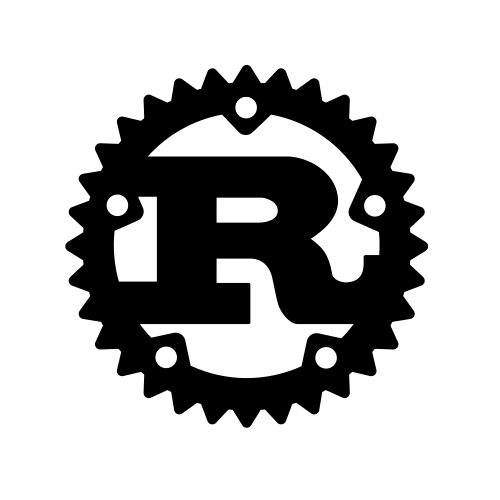
\includegraphics[height = \textheight]{rust_logo.png}%
      \end{onlyenv}
    \end{column}
  \end{columns}

  \note<1>{

    Я практически \textbf{не затронул параллелизм}!

    На Rust легко программировать надёжные системы. Да, я до сих пор буду
    совершать ошибки при разработке системы в целом, но зато мне не надо думать
    о целом классе других ошибок. Я могу полностью сконцентрироваться на
    архитектуре, на конечной цели.

  }

  \note<2>{

    Rust можно использовать для написание практически всего, чего угодно. Я вам
    приводил примеры того, для чего использовал Rust я, а также примеры того,
    где используют Rust крупные компании в production.

  }

  \note<3>{

    Rust объединяет в себе лучшее других языков, при этом оставляет за бортом
    плохое.

    \begin{itemize}
    \item Но безопасный и более юзабельный.
    \item Но без тяжёлого runtime.
    \item Но без GC и его проблем как таковых.
    \item Взято у других и улучшено.
    \end{itemize}

  }

  \note<4>{

    Благодаря системе владения, приходится писать код короче, быстрее, лёгким
    для понимания и изменения, хочу я этого или нет (иначе компилятор будет
    ругаться).

  }

  \note<5>{

    Я реально не встречал сообщества более лучшего, чем у Rust. Вы можете просто
    кинуть ссылку на Playground и попросить сделать code review. И вам его
    сделают, какой бы уровень у вас не был.

    Мейнтейнеры самые доброжелательные, многие пофиксят баги, которые ты
    попросишь, потому что писать на Rust в кайф, хочется, чтобы твой код был
    максимально чистым и рабочим.

  }

  \note<6>{

    Все тулы для Rust кажутся идиоматичными и составляют единое целое. Пока не
    попробуешь --- не поймёшь.

  }

  \note<7>{

    Что ни новая версия Rust --- то стабилизация какой-то крутой фичи. Многие
    языки программирования копируют концепции Rust.

    Заинтересовавшимся \textbf{могу накидать кучу ссылок}, где Rust описывается
    профессиональными разработчиками на C/C++, а также где Rust приходит на
    замену чего-либо (C/C++ или Python).

  }

\end{frame}

\begin{frame}[standout]
  \color{dWhite}Questions?
\end{frame}

\appendix

\begin{frame}[allowframebreaks]{References}

  % \nocite{*}

  \bibliographystyle{ieeetr}
  \bibliography{main}

\end{frame}

\end{document}
